\begin{comment}
\chapter{Belle II e acceleratore SKB (SuperKEKB)}
%\addcontentsline{toc}{chapter}{Belle II e acceleratore SKB (SuperKeKB)}
\end{comment}

\begin{comment}
Belle II è un esperimento general-purpose utilizzato nello studio dei parametri del Modello Standard (MS) e nella ricerca di Fisica oltre il MS (Beyond Standard Model, BSM).
In particolare l'esperimento studia la violazione di CP nei sistemi di mesoni B e cerca evidenze di Nuova Fisica (New Physic, NP) nei decadimenti dei mesoni B, dei mesoni D, nei leptoni $\tau$ e nel dark sector (settore della materia oscura), in particolare dei fotoni oscuri.
\end{comment}

%---------------------------------------------
%			1.1
%---------------------------------------------
\begin{comment}
\section{Programma di fisica alle B-Factory}
%\addcontentsline{toc}{section}{Programma di fisica alle B-Factory}
\end{comment}

\begin{comment}

Lo SM è una teoria che descrive tre delle interazioni fondamentali tra le particelle elementari, cioè l'interazione forte, debole ed elettromagnetica (ad esclusione quindi, della gravità).
Classifica tutte le particelle fino ad ora note, in 4 gruppi principali: quark, leptoni, bosoni e Higgs. 

\begin{figure}
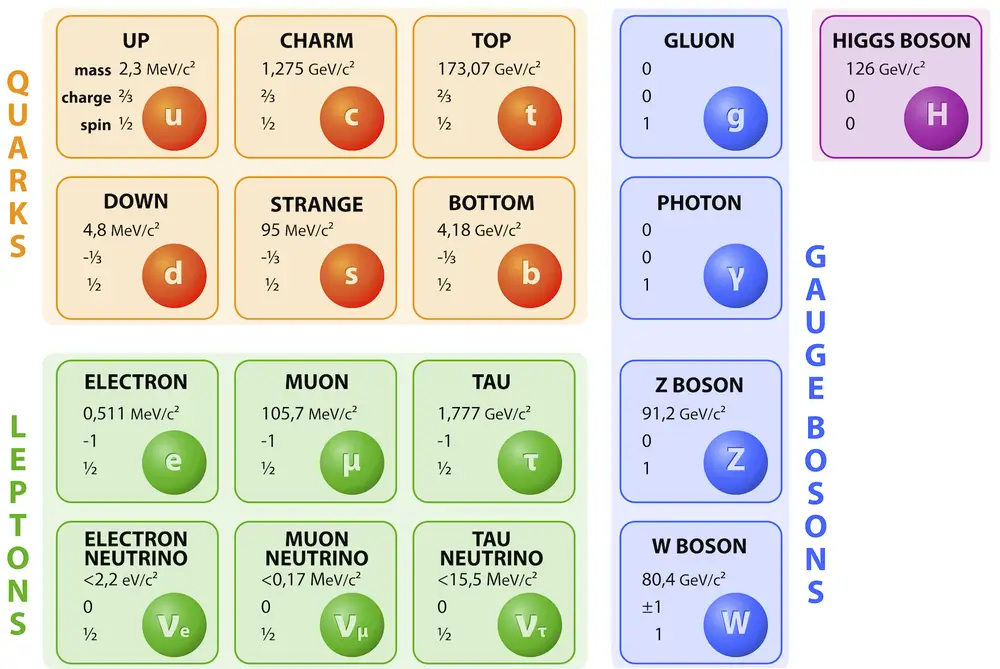
\includegraphics{SM}
\caption{Modello Standard}
\label{fig:sm}
\end{figure}

Nonostante abbia ottenuto negli anni una serie di sorprendenti successi, riuscendo a predire con precisione nuove particelle e nuovi meccanismi fino a quel momento sconosciuti, ci sono ancora numerosi e fondamentali aspetti della Natura sulla quale non è in grado di dare risposte. 

Si conoscono, ad esempio, tre generazioni di quark e leptoni ma non si sa se debbano essere i soli e non si conosce il perché della loro gerarchia di massa.
Il meccanismo di Higgs spiega la causa delle masse delle particelle elementari attraverso la rottura spontanea della simmetria elettrodebole, ma non giustifica quella dei neutrini. 
Lo SM inoltre potrebbe prevedere anche l'esistenza di altri bosoni Higgs-like, eventualmente vettoriali, la cui esistenza sarebbe giustificata in alcune teorie di Supersimmetria (SUSY) o altre di Nuova Fisica.
Un'ulteriore problema irrisolto è l'asimmetria tra materia e antimateria nell'universo. Nonostante la violazione di CP sia necessaria per spiegare l'attuale stato dell'universo, quella osservata è diversi ordini di grandezza minore, rispetto a quella necessaria per spiegare la dominazione della materia sull'antimateria, che ha permesso l'evoluzione dell'universo come lo osserviamo oggi. 
Inoltre, gli elementi della matrice di Cabibbo-Kobayashi-Maskawa (CKM), la cui fase complessa è alla base della violazione di CP nel settore dei flavor dei quark, sono diagonali e questo potrebbe suggerire l'esistenza di una nuova simmetria, che esiste non rotta ad elevate energie (superiori all'ordine del TeV).
Tutte queste questioni aperte, incentivano dunque la ricerca di nuove particelle e nuovi processi (meccanismi) che possano dare delle risposte.
Alla frontiera dell'energia, esperimenti com il Large Hadron Collider (LHC) a Ginevra, cercano nuove particelle prodotte nella collisione protone-protone fino ad una energia nel centro di massa di 14 TeV.
Alla frontiera della luminosità invece, la traccia di nuove particelle e meccanismi si cerca in misure di precisione nelle reazioni soppresse nella fisica del flavor o nelle deviazioni dalle predizioni del MS. Le discrepanze infatti, possono essere interpretate come indizio (segnale) di nuova fisica oltre il Modello Standard. Quest'ultimo è l'approccio di Belle II.
\end{comment}
\begin{comment}
\subsection{Ricerche di nuova fisica (BSM)}

\end{comment}
%%%%%%%%%%%%%%%%%%%%%%
%	PRIMO CASO DA PHYSICS BOOK
%%%%%%%%%%%%%%%%%%%%%%

\begin{comment}
In Belle II è possibile ricercare modelli di nuova fisica che includono specifici accoppiamenti di flavor, la cui ricerca indiretta potrebbe spingere la scala di energia di nuovi meccanismi a livelli anche più alti rispetto alla ricerca diretta, suggerendo inoltre, in quale direzione muoversi per scoprire eventuali nuovi processi. 

Un'importante transizione molto studiata in Belle II è \textit{b}$\rightarrow$\textit{s}. 
Inizialmente la misura di violazione di CP nei sistemi $B_{d}$ è stata fatta usando transizioni a tre livelli del tipo \textit{b}$\rightarrow$\textit{c\bar{c}s}, ad esempio nel golden channel B$\rightarrow$ J/$\psi$$K_{S}^{0}$. Successivamente si è cominciato ad osservare la violazione di CP anche nelle transizioni a loop indotto(??) \textit{b}$\rightarrow$\textit{s}, come B$\rightarrow$ $\phi$$K_{S}^{0}$ oppure B$\rightarrow$ $\eta'$$K_{S}^{0}$. Anche se l'attuale precisione possibile in questi canali, non raggiunge quella dei precedenti.

Nello MS la violazione di CP attesa in queste transizioni è abbastanza piccola, quindi qualsiasi osservazioni significativa potrebbe essere segnale di nuova fisica. 

Un ulteriore indizio di nuova fisica, è stato trovato negli anni passati nella misura del Branching-ratio di B$\rightarrow$ $\nu\tau$, che è una annichilazione a tre livelli del tipo \textit{b}$\rightarrow$\textit{u} e il cui stato finale include almeno due neutrini, per cui una sfida impegnativa dal punto di vista sperimentale.
\end{comment}

\begin{comment}
\subsection{Fisica del flavor}

\subsection{Materia oscura}


\end{comment}


%%%%%%%%%%%%%%%%%%%%%%
%	SECONDO CASO DA PHYSICS BOOK overview
%%%%%%%%%%%%%%%%%%%%%%










%---------------------------------------------
%			1.2
%---------------------------------------------
\begin{comment}
\section{Acceleratore SuperKEKB}
%\addcontentsline{toc}{section}{Acceleratore SuperKEKB}
\end{comment}

\begin{comment}
La sensibilità nelle misure di precisione alla ricerca di nuova fisica, sono possibili soprattutto grazie alla complessità e alle ottime prestazioni dell'acceleratore SuperKEKB che ospita il rivelatore ermetico Belle II. Risultato di molti anni di efficiente collaborazione tra i ricercatori del laboratorio KEK e tutte le collaborazioni internazionali che partecipano all'esperimento.

SuperKEKB è un collider asimmetrico $e^{+}e^{-}$ di 3 km di circonferenza, piccato a una energia del centro di massa pari a $\sqrt{s}$ = 10.58 GeV, che corrisponde alla massa della risonanza $\Upsilon(4S)$. 

Rispetto al suo predecessore KEKB, l'attuale acceleratore ha permesso di ottenere il primato di luminosità mai raggiunta, pari a ......, utilizzando uno schema differente nell'accelerazione e scontro dei fasci, attraverso alcune migliorìe e aggiunte nelle componenti fondamentali dell'acceleratore stesso.

\begin{figure}
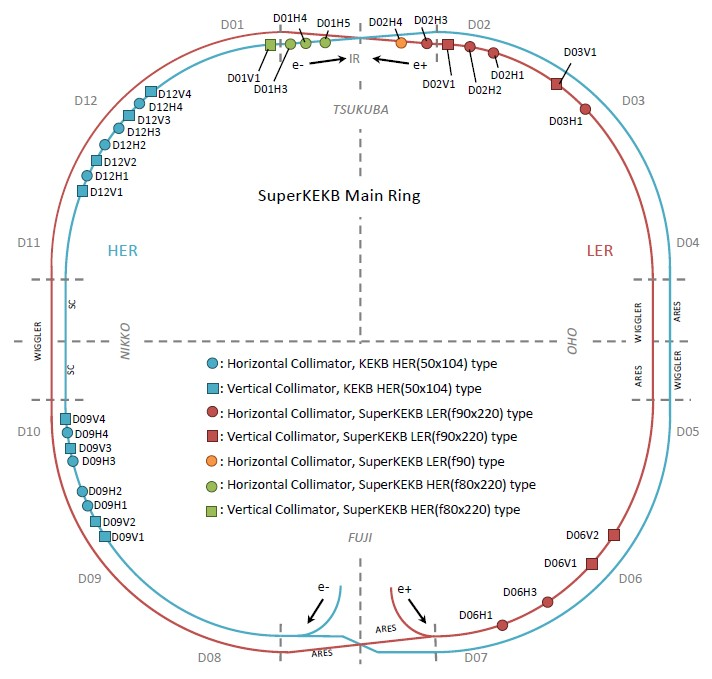
\includegraphics{SuperKEKB}
\caption{L'acceleratore SuperKEKB nel 2021. Le lettere V ed H indicano rispettivamente i collimatori verticali ed orizzontali. Ciascun anello è diviso in 12 sezioni, dalla prima chiamata D01 fino al'ultima D12.}
\label{fig:superkekb}
\end{figure}


(Andiamo attraverso le sue principali caratteristiche)
%%struttura meccanica(lunghezza, fasci, etc...)
\end{comment}

\begin{comment}
\subsection{Luminosità}
\end{comment}

\begin{comment}
Uno dei parametri cardine di un acceleratore è la luminosità, che rappresenta il rate di interazione per unità di sezione d'urto tra particelle che collidono:

\begin{equation}
L =\frac{1}{\sigma}\frac{dN}{dt} 
\end{eqaution}

da cui, invertendo la relazione per ricavare N, cioè il numero degli eventi fisici osservabili, si ottiene:

\begin{equation}
N = \int_{0}^{T} L\sigma dt
\end{equation}

dove T è la durata dell'esperimento, $\sigma$ la sezione d'urto del processo fisico d'interesse.
In generale la luminosità è strettamente dipendente dai parametri di macchina dell'acceleratore e dalle caratteristiche del fascio. Può essere espressa come:

\begin{equation}
L = ..................
\end{equation}

dove ......

L'attuale record mondiale detenuto da SuperKEKB è di 3.8$\dot 10^{34}$ $cm^{-2} s^{-1}$ con $\beta^{*}_{y}$= 1.0 mm. Il target nei prossimi anni è quello di raggiungere un picco di luminosità pari a 6.3 $\dot 10^{35}$ $cm^{-2} s^{-1}$, possibile aumentando le correnti dei fasci e riducendo la sezione degli stesi nel Punto d'Interazione (IP), strizzando la funzione di betatrone fino a un valore $\beta^{*}_{y}$= 0.3 mm.
La gestione del background dei fasci diventa una questione fondamentale in questo ambito, sia per raggiungere il target, sia per affinare le misure di fisica possibili. 

Attualmente si stima che il background dovrebbe rimanere accettabile fino ad una luminosità di 2,8$\dot 10^{35}$ $cm^{-2} s^{-1}$ con $\beta^{*}_{y}$= 0.6 mm. 
%METTI REFERENZA '' Beam bkg expectation (A)''

Come vedremo, la possibilità di raggiungere picchi più elevati di luminosità è strettamente legata a un piano di upgrade del rivelatore e di alcune componenti dell'acceleratore stesso.

\end{comment}

\begin{comment}
\subsection{Energia dei fasci}
\end{comment}

\begin{comment}

L'energia dei fasci è determinata dal programma di fisica interessante per l'esperimento. Attualmente SuperKEKB collide un fascio di elettroni di energia pari a 7 GeV (High Energy Ring, HER) con un fascio di positroni a 4 GeV (Low Energy Ring, LER), ottendendo un'energia nel centro di massa piccata alla risonanza $\Upsilon$(4S). 
Anche la scelta di utilizzare fasci asimmetrici in energia (come già il suo predecessore KEKB, che collideva fasci di elettroni a 8 GeV con fasci di positroni a 3.5 GeV) è necessaria per identificare e misurare i vertici di decadimento delle particelle create nella collisione. Questo meccanismo permette infatti di dare ai prodotti un boost, migliorando la ricostruzione dei vertici e quindi incrementando la sensibilità alle misure di fisica??????????????????????
%%VEDI COME E' NECESSARIO NELLE MISURE DI FISICA

In figura \vref{beame} è mostrata la flessibilità dell'energia di entrambi i fasci LER e HER. Il range possibile copre energie dalla $\Upsilon$(1S) alla $\Upsilon$(6S), con picco corrispondente a 11.24 GeV. 

\begin{figure}
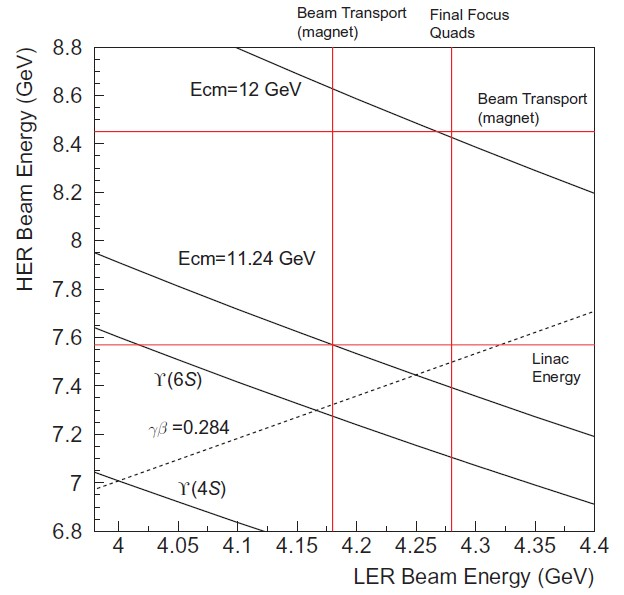
\includegraphics{beam_energy}
\caption{Nenergie dei fasci per raggiungere energie nel centro di massa pari a $\Upsilon$(4S), $\Upsilon$(6S),11.24 GeV e 12 GeV. L'asse orizzontale rappresenta l'energia del LER e quella verticale del HER. }
\label{fig:beame}
\end{figure}

\end{comment}

\begin{comment}
\subsection{Schema ''Nano-beam''}
\end{comment}

\begin{comment}
Come accennato nei paragrafi precedenti, un elemento chiave per definire la luminosità è la funzione beta $\beta$ nel PI. Per poter aumentare la luminosità è necessario diminuire il valore di $\beta$ compatibilmente con la variazione di tutti gli altri parametri di macchina e non, che rientrano nella sua definizione. 
In particolare, lo schema dei fasci utilizzato in SuperKEKB è chiamato \textit{nano-beam scheme}, e ha permesso di ottenere una luminosità 40 volte maggiore di quella del predecessore KEKB (che ha operato dal....al 2011), riuscendo a ridurre di 1/20 la funzione $\beta$ nel PI. 

Questo nuovo schema, ideato da P. Raimondi, prevede che i fasci collidano a grande angolo, in SuperKEKB pari a 83 mrad, (mantenendo i fasci separati tramite quadrupoli magnetici) per poter ridurre l'hourglass effect, che subentra per bunch di particelle molto lunghi all'interno del fascio. (Vediamo i parametri fondamentali che influenzano la scelta.)
L'area di sovrapposizione dei fasci è localizzata e la sua lunghezza è data da:

\begin{equation}
d = \frac{\sigma_{x}^{*}}{sin\phi_{x}}
\end{equation}

con $\phi_{x}$ definito come metà dell'angolo di crossing. La lunghezza di overlap d, rappresenta la vera lunghezza del bunch da considerare nella ``valutazione'' dell'effetto clessidra, ed è più piccola dell'effettiva lunghezza del bunch lungo la direzione dell'asse del fascio. Per ridurre l'effetto clessidra, è necessario avere:

\begin{equation}
\beta_{y}^{*} \geq d = \frac{\sigma_{x}^{*}}{sin\phi_{x}}
\end{equation}

Dunque per aumentare la funzione $\beta$ nel PI, è necessario diminuire il valore di d, facendo decrescere la sezione orizzontale nel PI e aumentando l'angolo di crossing.
Utilizzare un angolo di crossing abbastanza grande, ha altre implicazioni positive sul funzionamento dell'acceleratore:

\begin{item}
\item permettel'installazione di un nuovo sistema di focusing nel PI con un quadrupolo magnetico superconduttore;
\item permette di avere due linee separate che ospitano i fasci HER e LER;
\item diminuisce l'effetto dei ''fringe fields'' nel PI, che sono residui dei magneti nelle vicinanze. 
\end{item}

%%%%%% CRAB WAIS COLLISION SCHEME
In figura \ref{fig:beampar} si riportano i parametri di macchina (default) dell'acceleratore SuperKEKB.

\begin{equation}
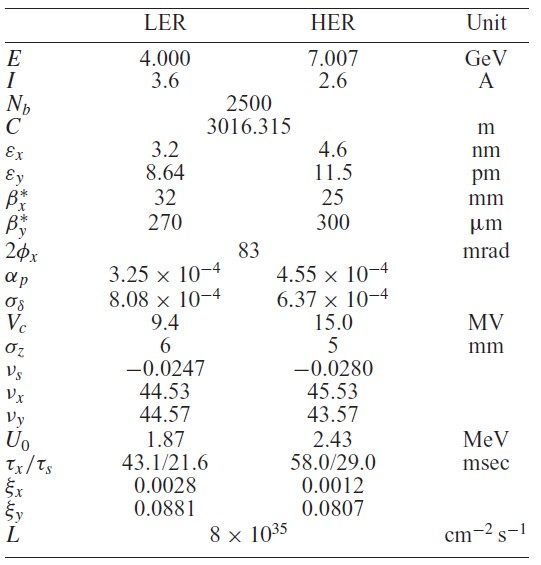
\includegraphics{beam_par}
\caption{Parametri di macchina di SuperKEKB. Il simbolo ''*'' indica i valori nel PI.}
\label{fig:beampar}
\end{equation}

%PARLARE DELLA COSA ORIZZONTALE???

\end{comment}


\begin{comment}
\subsection{Cromaticità e correzioni ottiche}
%SECONDO ME NO

\subsection{Iniezione}
%BHO

\subsection{Alcune ulteriori modifiche rispetto a KEKB}
\end{comment}

\begin{comment}

L'upgrade da KEKB a SuperKEKB, come in parte visto, ha richiesto importanti cambiamenti nei fasci e nello schema di collisione, tutto volto a raggiungere nuove vette di luimnosità. Altre fondamentali modifiche sono state fatte lungo l'anello di collisione, tra cui:

\begin{item}
\item rifacimento della regione d'interazione, che comprende 4 m intorno al PI, in modo da poter ospitare il nuovo detector Belle II, il sistema di focusing finale dei fasci e le due beam pipes;
\item il sistema a radiofrequenza è stato modificato per permettere una corrente maggiore dei fasci;
\item l'aggiunta di alcuni collimatori lungo entrambi gli anelli (11 nel LER  e 20 nel HER) per poter limitare il danno da radiazione sul rivelatore e i ''quenches'' dei magneti superconduttori, cioè un surriscaldamento dei suoi avvolgimenti che genericamente causa la perdità della superconduttività, dissipando la corrente circolante.
\item anche il sistema di vuoto è stato migliorato per limitare alcuni effetti collegati alla perdita di potenza del fascio, allungando quindi la vita media del fascio stesso.
\end{item}

\end{comment}

\begin{comment}
\subsection{Sistemi di monitoraggio del background}
\end{comment}%% Per le sorgenti di rumore si rimanda al capitolo 2 o lo metti nel capitolo 2?


\begin{comment}
Il background è una delle principali problematiche di un rivelatore, sia per le misure di precisione di fisica, sia per le performance dei vari strati rivelatori di cui è formato Belle II.
A tal ragione, vengono utilizzati diversi rivelatori per poter avere misure della dose di radiazione sia sul rivelatore che su zone delicate dell'acceleratore, per poter intervenire quanto prima in caso di livelli troppo elevati. Grandi dosi di radiazione infatti, posso causare danni accidentali sul rivelatore, diminuendone le performance.??????????????????????
Tra i principali (?) ci sono:

\begin{itemize}
\item Detector di diamante (chiamati ''Diamanti'') che monitorano il rate della dose di radiazione nella zona d'interazione della beam pipe. Questi rientrano anche nel ''fast beam abort system'', cioè un sistema di controllo che considera dati di diversi detector per poter valutare lo ''spegnimento'' dei fasci, per evitare che situazioni fuori controllo arrechino danni a tutta la struttura.
\item il CLAWS (sCintillation Light And Waveform Sensors), formato da scintillatori di materiale plastico e fotomoltiplicatori di silicio, usato per monitorare il background di Belle II in corrispondenza dell'iniezione del fascio (nell'anello principale). Con i diamanti fa parte della logica del sistema di aborto del fascio.
\item TPC's (Time Projection Chambers) che fornisce misure sulla direzione del flusso dei neutroni nel tunnel che ospita l'acceleratore.
\item Tubi di $He^{3}$ per il conteggio dei neutroni termici (con energie cinetiche inferiori a 1/10 di eV, generalmente intorno a 0.025 eV) intorno al rivelatore Belle II.
\end{itemize}

\end{comment}
%---------------------------------------------
%			1.3
%---------------------------------------------
\begin{comment}
\section{Il rivelatore Belle II}
%\addcontentsline{toc}{section}{Il rivelatore Belle II}
\end{comment}

\begin{comment}
Il rivelatore Belle II è uno spettrometro di particelle general-purpose, ottimizzato nelle misure di precisione dei mesoni B e dei loro prodotti di decadimento. Rispetto al suo predecessore Belle, deve riuscire a mantenere buone performance, pur avendo un minore boost nel centro di masse e nonostante sia sottoposto a maggiori livelli di background e quindi di radiazione, che sono la principale causa di una prematura degradazione delle prestazioni e della vita media del rivelatore stesso.

Belle II consiste in una serie di sottorivelatori annidiati, che circondano il PI dei due fasci, posti intorno alla beam pipe di berillio di 1cm di raggio.

\end{comment}

\begin{comment}
\subsection{Vertex Detector (VXD)}

\subsection{Central Drift Chamber (CDC)}

\subsection{Particle identification system (TOP e ARICH)}

\subsection{Calorimetro elettromagnetico (ECL)}

\subsection{$K_{L}$ muon detector (KLM)}

\subsection{Sistema di trigger}


%---------------------------------------------
%			1.4
%---------------------------------------------
\section{Stato attuale e prospettive delle prese dati}
%\addcontentsline{toc}{section}{Stato attuale e prospettive delle prese dati}

%%%% 	Luminosità raggiunte e statistica?
%%Belle II online luminosity & record luminosità istantanea
%% doev si vuole arrivare 50 abinv e come??
%% cose achved nelle previsioni parametri di macchina dell'articolo B

%ARTICOLO B: there are two major upgrades of the machine plannd in the next ten years:....
\end{comment}